\setcounter{chapter}{0}
\setcounter{section}{0}
\begin{center}
\chapter{\tenchuongi}
\end{center}

%===================================================================
\section{Khái quát về CNN}
\subsection{Giới thiệu}
\begin{figure}[H]
	\centering
	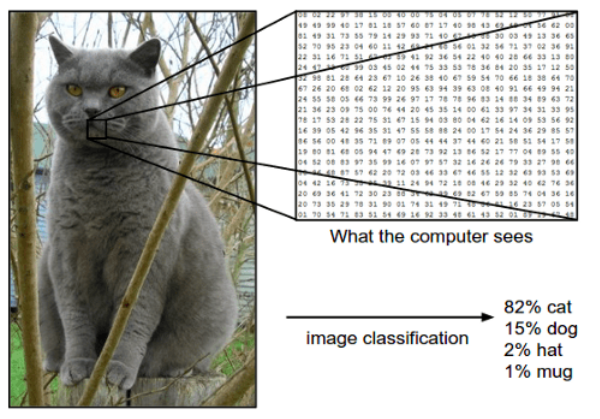
\includegraphics[width=1\linewidth]{images/how_computer_see_image}
	\caption[Cách máy tính "nhìn" một hình.]{Cách máy tính "nhìn" một hình ảnh.}
	%\label{fig:howcomputerseeimage}
\end{figure}

Convolutional Neural Networks (CNN) là một trong những mô hình deep learning phổ biến nhất và có ảnh hưởng nhiều nhất trong cộng đồng Computer Vision. CNN được dùng trong trong nhiều bài toán như nhân dạng ảnh, phân tích video, ảnh MRI, hoặc cho bài các bài của lĩnh vự xử lý ngôn ngữ tự nhiên, và hầu hết đều giải quyết tốt các bài toán này.

Mạng CNN lấy cảm hứng từ não người \cite{cnnhumanbrain}. Nghiên cứu trong những thập niên 1950 và 1960 của D.H Hubel và T.N Wiesel trên não của động vật đã đề xuất một mô hình mới cho việc cách mà động vật nhìn nhận thế giới. Trong báo cáo, hai ông đã diễn tả 2 loại tế bào neural trong não và cách hoạt động khác nhau: tế bào đơn giản (simple cell – S cell) và tế bào phức tạp (complex cell – C cell). 

Năm 1980, Fukushima đề xuất mô hình mạng neural có cấp bậc gọi là neocognitron. Mô hình này dựa trên khái niệm về S cell và C cell. Mạn neocognitron có thể nhận diện mẫu dựa trên việc học hình dáng của đối tượng. 

Sau đó vào năm 1998, mạng CNN được giới thiệu bởi Bengio, Le Cun, Bottou và Haffner. Mô hình đầu tiên của họ được gọi tên là LeNet-5. Mô hình này có thể nhận diện chữ số viết tay.

\subsection{Kiến trúc mạng CNN}
Mạng CNN gồm hai thành phần:

\indent\indent \textbf{Phần tầng ẩn hay phần rút trích đặc trưng:} trong phần này, mạng sẽ tiến hành tính toán hàng loạt phép tích chập và phép hợp nhất (pooling) để phát hiện các đặc trưng.

\indent\indent  \textbf{Phần phân lớp:} tại phần này, một lớp với các liên kết đầy đủ sẽ đóng vai trò như một bộ phân lớp các đặc trưng đã rút trích được trước đó. Tầng này sẽ đưa ra xác suất của một đối tượng trong hình \ref{fig:kientruccnn}.
\begin{figure}[H]
	\centering
	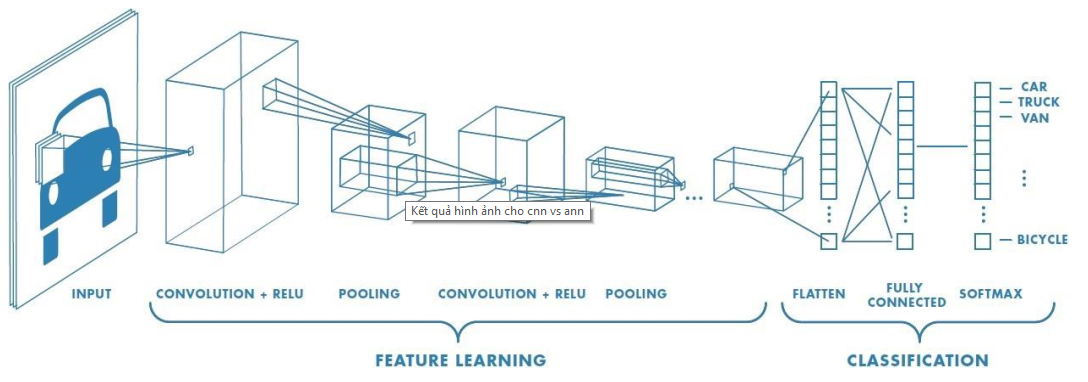
\includegraphics[width=1\linewidth]{images/kientruccnn}
	\caption{Kiến trúc mạng CNN.}
	\label{fig:kientruccnn}
\end{figure}

\subsubsection{Trích rút đặc trưng}
\paragraph{Lớp tích chập}
Tích chập là một khối quan trọng trong CNN. Thuật ngữ tích chập được dựa trên một phép hợp nhất toán học của hai hàm tạo thành hàm thứ ba. Phép toán này kết hợp hai tập thông tin khác nhau.

Trong trường hợp CNN, tích chập được thực hiện trên giá trị đầu vào của dữ liệu và kernel/filter (thuật ngữ này được sử dụng khác nhau tùy tình huống) để tạo ra một bản đồ đặc trưng (feature map). 

Ta thực hiện phép tích chập bằng cách trượt kernel/filter theo dữ liệu đầu vào. Tại mỗi vị trí, ta tiến hành phép nhân ma trận và tính tổng các giá trị để đưa vào bản đồ đặc trưng. Thao tác này đã được minh họa cụ thể trong hình \ref{fig:padding18}

\begin{figure}[H]
	\centering
	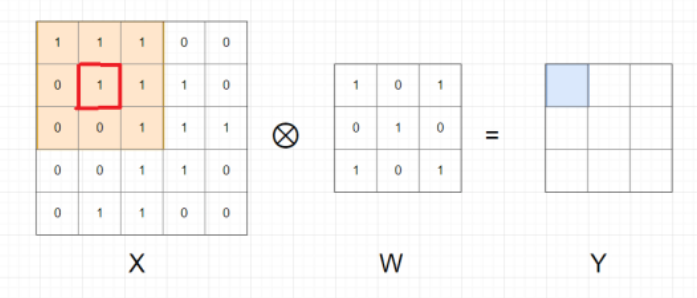
\includegraphics[width=1\linewidth]{images/padding18.png}
	\caption{Minh họa phép tích chập.}
	\label{fig:padding18}
\end{figure}

\paragraph{Lớp ReLU}

Tương tự như mạng neural thông thường, ta sử dụng một hàm kích hoạt (activate function) để có đầu ra dưới dạng phi tuyến. Trong trường hợp CNN, đầu ra của phép tích chập sẽ đi qua hàm kích hoạt nào đó ví dụ như hàm tinh chỉnh các đơn vị tuyến tính (Rectified linear units - ReLU). 

\paragraph{Lớp pooling}

Thông thường, sau mỗi tầng tích chập, ta sẽ cho kết quả đi qua một tầng hợp nhất (pooling layer). Mục đích của tầng này là để nhanh chóng giảm số chiều. Việc này giúp giảm thời gian học và hạn chế việc overfitting. 


Như vậy, khi thiết kế phần rút trích đặc trưng của mạng CNN, ta cần chú ý đến 4 siêu tham số quan trọng là: Kích thước kernel/filter, Số lượng kernel/filter, Kích thước bước nhảy (stride), Kích thước lề (padding).

\subsubsection{Phân lớp}
Tầng cuối cùng trong mạng CNN là một tầng liên kết đầy đủ, phần này hoạt động tương tự như mạng neural thông thường. Kết quả thu được cuối cùng cũng sẽ là một véc-tơ với các giá trị xác suất cho việc dự đoán như mạng neural thông thường.

\subsection{Ứng dụng CNN trong phân loại ảnh}
Các bước để thực hiện phân loại hình ảnh dựa trên mạng CNN được mô tả trong Hình \ref{fig:placnn}. Đầu tiên, kho dữ liệu ảnh đầu vào được nạp. Ảnh này được chia làm hai phần, một phần dành cho luyện mạng và một phần cho kiểm tra. Trước tiên, ta phải lựa chọn cấu trúc mạng CNN bao gồm số lượng lớp ẩn, các tham số trong mỗi lớp ẩn như kích thước trường tiếp nhận cục bộ, stride, padding.  Ảnh luyện mạng sau đó được đưa vào lớp chập 1 để thực hiện tích chập trên ảnh và thực hiện hàm ReLU. Sau đó, kết quả được đưa đến quá trình thực hiện pooling với tham số pooling size phù hợp để giảm kích cỡ ảnh. Ảnh sẽ tiếp tục được đưa thêm qua các lớp tích chập nữa cho đến khi đạt được kết quả mong muốn. Kết quả này được dàn phẳng và đưa vào lớp kết nối đầy đủ. Cuối cùng là quá trình thực hiện các activation function và phân loại ảnh. Quá trình luyện mạng sẽ kết thúc sau khi tổng sai số nhỏ hơn một ngưỡng cho phép hoặc sau một số thế hệ cho trước (điều kiện hội tụ). Kết thúc của quá trình luyện mạng là cấu trúc mạng CNN với các tham số phù hợp. Để kiểm tra, các mẫu ảnh kiểm tra được đưa qua mạng CNN rồi thực hiện đánh giá sai số.

\subsubsection{Trường tiếp nhận cục bộ (Local receptive fields)}
Là một cửa sổ nhỏ trên các điểm ảnh đầu vào. Mỗi kết nối sẽ học một trọng số và neural ẩn cũng sẽ học một độ lệch (overall bias). Ta có thể hiểu rằng, neural lớp ẩn cụ thể học để phân tích trường tiếp nhận cục bộ cụ thể của nó.

Có thể thấy rằng, trường tiếp nhận cục bộ thích hợp cho việc phân tách dữ liệu ảnh, giúp chọn ra những vùng ảnh có giá trị nhất cho việc đánh giá phân lớp.

\subsubsection{Trọng số chia sẻ và độ lệch (Shared weights and biases)}
Chúng ta gọi việc map từ input layer sang hidden layer là một feature map. Ta cần tìm ra mối quan hệ giữa số lượng Feature map với số lượng tham số.

Chúng ta thấy mỗi fearture map cần 25 = 5×5 shared weight và 1 shared bias. Như vậy mỗi feature map cần 5×5+1 = 26 tham số. Như vậy nếu có 10 feature map thì có 10×26 = 260 tham số. Chúng ta xét lại nếu layer đầu tiên có kết nối đầy đủ nghĩa là chúng ta có 28×28=784 neural đầu vào như vậy ta chỉ có 30 neural ẩn. Như vậy ta cần 28x28x30 shared weight và 30 shared bias. Mô hình có số lượng tham số ít hơn thì nó sẽ chạy nhanh hơn.

\subsubsection{Lớp chứa hay lớp tổng hợp (Pooling layer)}
Ngoài các lớp tích chập vừa mô tả, mạng neural tích chập cũng chứa các lớp pooling. Lớp pooling thường được sử dụng ngay sau lớp tích chập. Những gì các lớp pooling làm là đơn giản hóa các thông tin ở đầu ra từ các lớp tích chập. 

Chúng ta có thể hiểu max-pooling như là một cách cho mạng để hỏi xem một đặc trưng nhất được tìm thấy ở bất cứ đâu trong một khu vực của ảnh. Sau đó nó bỏ đi những thông tin định vị chính xác. Trực giác là một khi một đặc trưng đã được tìm thấy, vị trí chính xác của nó là không quan trọng như vị trí thô của nó so với các đặc trưng khác. Một lợi ích lớn là có rất nhiều tính năng gộp ít hơn (fewer pooled features), và vì vậy điều này sẽ giúp giảm số lượng các tham số cần thiết trong các lớp sau.

\subsubsection{Cách chọn tham số cho CNN}
Hiệu quả hoạt động của mạng CNN phụ thuộc rất nhiều vào việc lựa chọn các tham số sau:

\begin{itemize}
	\item Số các convolution layer: càng nhiều các convolution layer thì performance càng được cải thiện. Sau khoảng 3 hoặc 4 layer, các tác động được giảm một cách đáng kể.
	\item Filter size: thường filter theo size 5×5 hoặc 3×3
	\item Pooling size: thường là 2×2 hoặc 4×4 cho ảnh đầu vào lớn
\end{itemize}

Trong thực tế, tùy vào ứng dụng cụ thể mà ta chọn các tham số khác nhau. Thông thường ta sẽ thực hiện nhiều lần việc train test để chọn ra được param tốt nhất (Phương pháp thử sai).

\section{Bài toán chuẩn đoán bệnh lao}
\subsection{Các dữ liệu để chuẩn đoán bệnh lao}
Để chuẩn đoán được bệnh lao cần dựa vào rất nhiều dữ liệu \cite{bytchuandoanlao} như: 
\begin{itemize}
	\item {\bfseries Lâm sàng}
	\begin{itemize}
		\item {\bfseries Toàn thân:} Sốt nhẹ về chiều, ra mồ hôi đêm, chán ăn, mệt mỏi, gầy sút cân.
		\item {\bfseries Cơ năng:} Ho, khạc đờm, ho ra máu, đau ngực, khó thở.
		\item {\bfseries Thực thể:} Nghe phổi có thể có tiếng bệnh lý (ran ẩm, ran nổ,....).
	\end{itemize}
	\item {\bfseries Cận lâm sàng}
	\begin{itemize}
		\item Nhuộm soi đờm trực tiếp tìm AFB.
		\item Xét nghiệm Xpert MTB/RIF (nếu có thể).
		\item Nuôi cấy tìm vi khuẩn lao.
		\item X-Quang phổi thường quy.
	\end{itemize}
\end{itemize}

Tuy vậy, do mục tiêu, đối tượng nghiên cứu, phạm vi nghiên cứu, nên luận văn chỉ tập trung nghiên cứu hỗ trợ chuẩn đoán bệnh lao qua các hình ảnh x-quang phổi thường quy dựa vào học máy, học sâu.

\subsection{Mô tả bài toán}
Như đã đề cập ở trên, luận văn chỉ tập trung nghiên cứu hỗ trợ chuẩn đoán bệnh lao qua các hình ảnh x-quang phổi thường quy dựa vào học máy, học sâu nên bài toán này chính là bài toán phân loại ảnh trong Thị giác Máy - Computer Vision.

Bài toán phân loại hình ảnh của luận văn là một trong những nhiệm vụ phổ biến trong Computer Vision. Mục tiêu chính của bài toán này đó chính là phân loại một hình ảnh đầu vào (input) thành một nhãn (label) đầu ra (output).  

Sau đó, ta sẽ tiến hành huấn luyện các mô hình học sâu của luận văn. Sau khi hoàn thành quá trình huấn luyện, ta có thể để các mô hình đã được huấn luyện kể trên thực hiện nhiêm vụ phân loại, dự đoán về khả năng ảnh x-quang phổi được đưa vào là của người có lao hay không, đây là nhãn (label) đầu ra (output) mong muốn cho bài toán của luận văn, dựa vào nhãn đầu ra ta sẽ kết luận xem người có ảnh chụp x-quang đó có bị lao hay tổn thương phổi không. 